\chapter{Implementation}
This chapter introduces the implementation of the multi-robot system. Chapter \ref{sec:communication_protocols} presents how communication among fixed sensors, charging stations, robots, and the centralized pool. Chapter \ref{sec:database} introduces different tables in database. Chapter \ref{sec:task_scheduling_procedure} describes the workflow of each component in the system


\section{Communication Protocols}
\label{sec:communication_protocols}

In the office environment, the centralized pool, robots, charging stations, and sensors need to share information. The centralized pool is the global controller in the multi-robot system. It can receive and learn room occupation from the robot and make decisions base on the information. The following are the way they communicate.

The robots can gather room occupation information while performing tasks. As long as the robot enters the sensor range, they conduct a rapid exchange of room occupation information. The robot then sends acquired room occupation data to the centralized pool. The centralized pool is the global controller that receives information about the robots and the environment and make decisions base on the information. The centralized pool uses this information in two ways. It assigns robots the navigation tasks according to the information and can assign robots to explore the room lacking the information. Once the robot finished current tasks, it notifies the central pool that the task is succeeded and requests a task from the centralized pool.

\subsection{Message about Measurement}
\label{sec:measurement_message}
When a robot passes by a door, it should receive messages from a sensor. In this project, we use a ROS node "sensor simulator" to simulate door sensors (Chapter \ref{sec:sensor_simulation}) to publish instant measurement result (Table \ref{tab:sensor_message}).

These Communication protocols save unnecessary communication costs by avoiding keep tracking the current position, availability, and states of all robots (Figure \ref{fig:communication_robot_pool}).

\begin{table}
\centering
\begin{tabular}{|c|c|c|c|c|} 
\hline
Door ID & Position& Timestamp & Measurement Result \\
\hline\hline
1&(-18.5,5.2) & 2020-06-01 9:00:02 & Door opened \\ [1ex] 
\hline
\end{tabular}
\caption{Measurement Message Format and Example}
\label{tab:sensor_message}
\end{table}
 

\subsection{Message about Task}
\label{sec:task_message}
There are some basic requirements for communication between the robot and centralized pool: firstly, the robot should initiate the communication once the task queue becomes empty. 
Secondly, the robot should forward sensor data to the centralized pool immediately after interacting with sensors. 
Four types of message are defined: 
(1) Task request message (Table\ref{tab:request_message}); (2) Task goal messages (Table \ref{tab:goal_message}); (3) Task feedback message (Table \ref{tab:feedback_message}); (4) Task result message (Table \ref{tab:result_message}). 

\begin{figure}
 \centering
 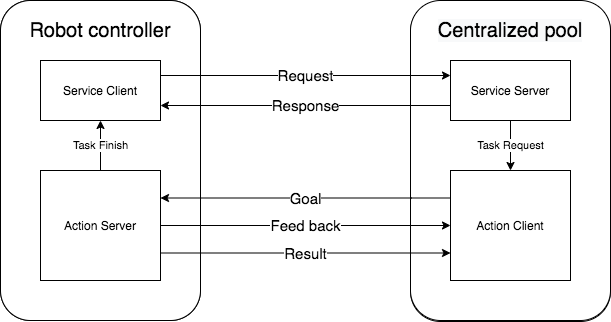
\includegraphics[width = 0.7\textwidth]{content/images/ch4/robot_pool_comminication.drawio.png}
 \caption{Communication between Robot and Centralized Pool}
 \label{fig:communication_robot_pool}
\end{figure}

\begin{table}
\centering
\begin{tabular}{|c|c|c|} 
\hline
Battery Level & Position & Robot ID\\
\hline\hline
93 &(2,4) &1 \\ [1ex] 
\hline
\end{tabular}
\caption{Request Message Format and Example}
\label{tab:request_message}
\end{table}

\begin{table}
\centering
\resizebox{\textwidth}{!}{
\begin{tabular}{|c|c|c|c|} 
\hline
Task ID-[] &Task type & Target ID & Goal[] \\
\hline\hline
1& Gather information task & 9 & (-1.5,5.2) 2020-06-01 9:00:00 \\
\hline
[3,4] & Navigation task & 21, 22 & (-24.0,12.0), 2020-06-01 9:02:00 (-21.0,12.0) 2020-06-01 9:02:00 \\
\hline
5 & Charging & 17 &(0.0,5.0), 2020-06-01 9:04:00 \\ [1ex] 
\hline
\end{tabular}}
\caption{Action Goal Message Format and Example}
\label{tab:goal_message}
\end{table}

\begin{table}
\centering
\begin{tabular}{|c|c|c|c|} 
\hline
Robot ID & Door ID & Measurement time & Measurement result \\
\hline\hline
1 & 3 & 2020-06-01 9:00:03 & Door open \\ 
1 & 4 & 2020-06-01 9:00:13 & Door open \\ 
1 & 5 & 2020-06-01 9:00:23 & Door open \\ 
\hline
\end{tabular}
\caption{Action Feedback Message Format and Example}
\label{tab:feedback_message}
\end{table}

\begin{table}
\centering
\begin{tabular}{|c|c|c|} 
\hline
Task ID & Task type & Result\\
\hline\hline
1 & Gather information task & Success \\ [1ex] 
\hline
\end{tabular}
\caption{Action Result Message Format and Example}
\label{tab:result_message}
\end{table}


\begin{table}
\centering
\begin{tabular}{|c|c|c|} 
\hline
Robot ID & Battery Level \\
\hline\hline
1 & 93 \\ [1ex] 
\hline
\end{tabular}
\caption{Message to Charging Station}
\label{tab:message_to_charging_staion}
\end{table}

\subsection{Message about Charging}
 
When a robot arrives charging station's position, it sends a message to Charging station(Figure \ref{tab:message_to_charging_staion}). The details of charging station is discussed in Chapter \ref{sec:charging_station}. 

\section{Database}
\label{sec:database}
The centralized pool keep environment information in database to make decisions. The structure of database is shown in Figure \ref{fig:database_er}.

\subsection*{Table tasks}
\begin{itemize}
 \label{sec:task_table}
 \item \textbf{Task ID.} A unique task identification.
 \item \textbf{Task Name.} Tasks names are ``gather enviroment information task '', ``navigation tasks'' or ``charging task''.
 \item \textbf{Start Time.} The start time refers to when the robot should move towards the target. A starting time is given when the task is created. This time can be a time in the future or empty (no time limit). 
 \item \textbf{Finish Time.} The default value is empty. When the centralized pool receives task result, this  will be updated to the time when the centralized pool received the result.
 \item \textbf{Target ID.} Targets include doors, points and charging stations. When a robot run a ``gather information task'', it moves to the front of a door and interact with a sensor in the door position without entering the door. 
 When robot run an ``navigation tasks'', the robot moves to a given point ether in corridor or in the room. When robot runs a ``charging task'', it moves to a charging station and interact with this charging station.
 \item \textbf{Robot ID.} A unique robot identification.
 \item \textbf{Priority.} Task priorities allow user to easily prioritize tasks to clearly plan what to do next. The ``charging tasks'' are given the highest priority of 5. The ``gather information tasks'' are given the lowest priority of 1. The ``navigation taskss'' has priority between 2-4 in the ``created'' status. Once this task failed once, its priority will be increased by 1 until it exceeds the maximum and is marked as ``Failed'' (Figure \ref{fig:centralized_task_handle}).
 \item \textbf{Task Status.} Task status are ``Created'', ``Succeeded'', ``Failed'', ``To rerun'', ``Error''. The difference between task status is discussed in Figure \ref{fig:centralized_task_handle}
 \item \textbf{Dependency.} If task B has a dependency of task A, task A needs to be preceded by tasks B. Those dependent tasks should be composed in the centralized pool.
 \item \textbf{Description.} The description of a succeeded task is ``succeeded''. The description of a failed task is its failure reason.
 \begin{table}
 \centering
 \resizebox{\textwidth}{!}{
 \begin{tabular}{|c|c|c|c|c|c|c|c|c|c|} 
 \hline
 Task ID & Task Type & Start Time & Target ID & Robot ID & Priority & Status & dependency & Finish Time & Description \\
 \hline
 1 & Charging task & 2020-06-01 9:00:00 & 18 & 1 & 5 & Succeeded & 0 & 2020-06-01 9:00:20 & Succeeded \\
 \hline
 2 & Navigation task & 2020-06-01 9:00:50 & 22 & 2 & 2 &Succeeded & 0 & 2020-06-01 9:01:20 & Succeeded \\
 \hline
 3 & Gather information task & 2020-06-01 9:02:00 & 2 & 2 & 1 & Running & 0 & 2020-06-01 9:02:40 & Succeeded \\ [1ex] 
 \hline
 \end{tabular}}
 \caption{Task Table in Database}
 \label{tab:db_task_table}
 \end{table}
\end{itemize}

\subsection*{Table measurements}
\begin{itemize}
 \item \textbf{Door ID.} Unique identification of the door.
 \item \textbf{Door Status.} Value 0 represent door closed. Value 1 represent door opened.
 \item \textbf{Date Time.} Measuring time.
 \begin{table}
 \centering
 \begin{tabular}{|c| c| c|} 
 \hline
 Door ID & Door Status & Date Time \\
 \hline
 9 & 1 & 2020-06-01 09:05:39 \\ \hline
 1 & 0 & 2020-06-01 09:05:49 \\ \hline
 7 & 1 & 2020-06-01 09:05:49 \\ \hline
 9 & 1 & 2020-06-01 09:05:49 \\ \hline
 1 & 1 & 2020-06-01 09:05:59 \\ \hline
 7 & 1 & 2020-06-01 09:05:59 \\ \hline
 9 & 1 & 2020-06-01 09:05:59 \\ \hline
 7 & 1 & 2020-06-01 09:06:09 \\ \hline
 16 & 0 & 2020-06-01 09:06:29 \\ \hline
 7 & 1 & 2020-06-01 09:06:39 \\ \hline
 16 & 1 & 2020-06-01 09:06:39 \\ \hline
 9 & 1 & 2020-06-01 09:06:49 \\ \hline
 8 & 0 & 2020-06-01 09:06:59 \\ \hline
 ... & ...& ... \\ \hline
 \end{tabular}
 \caption{Table measurements}
 \label{tab:db_measurement_result}
 \end{table}
\end{itemize}

\subsection*{Table door open possibilities}
\begin{itemize}
 \item \textbf{Door ID.} Unique identification of the door. 
 \item \textbf{Day of Week} a weekday.
 \item \textbf{Start Time and End Time} a time slot between start time and end time.
 \item \textbf{Initialized Open Probability} Predefined value to used to simulate door sensors (Chapter \ref{sec:sensor_simulation}).
 \item \textbf{Open Probability Statistic} Statistics of measurement result in the weekday and time slot.
 \begin{table}
 \centering
 \resizebox{\textwidth}{!}{
 \begin{tabular}{|c|c| c| c| c| c|} 
 \hline
 Door ID & Day Of Week & Start Time & End Time & Initialized Open Probability & Open Probability Statistic \\ \hline
 1 & 2 & 9:00:00 & 9:59:59 & 0.90 & 0.85 \\ \hline
 1 & 2 & 10:00:00 & 10:59:59 & 0.90 & 0.92 \\ \hline
 1 & 2 & 11:00:00 & 11:59:59 & 0.10 & 0.05 \\ \hline
 ...&...& ...&...&...&...\\ \hline
 \end{tabular}}
 \caption{Door Open Probability.}
 \label{tab:db_open_possibilities}
 \end{table}
\end{itemize}

\subsection*{Table doors}
\begin{itemize}
 \item \textbf{Door ID} Unique identification of door.
 \item \textbf{Last Update} The timestamp of last measurement result on the door.
 \item \textbf{Is Used} Value 1 represent at least one other robot is moving to this door. Value 0 represents no robot is moving to this door.
 \begin{table}
 \centering
 \begin{tabular}{|c|c|c|} 
 \hline
 Door ID & Last Update & Is Used \\ \hline
 1 & 2020-06-01 15:15:26 & 0 \\ \hline
 2 & 2020-06-01 15:15:06 & 0 \\ \hline
 3 & 2020-06-01 15:12:36 & 0 \\ \hline
 4 & 2020-06-01 15:15:16 & 0 \\ \hline
 5 & 2020-06-01 15:11:46 & 0 \\ \hline
 6 & 2020-06-01 15:11:36 & 1 \\ \hline
 7 & 2020-06-01 15:14:26 & 0 \\ \hline
 ...& ...& ... \\ \hline
 \end{tabular}
 \caption{Doors Table.}
 \label{tab:db_doors}
 \end{table}
\end{itemize}


\begin{figure}
 \centering
 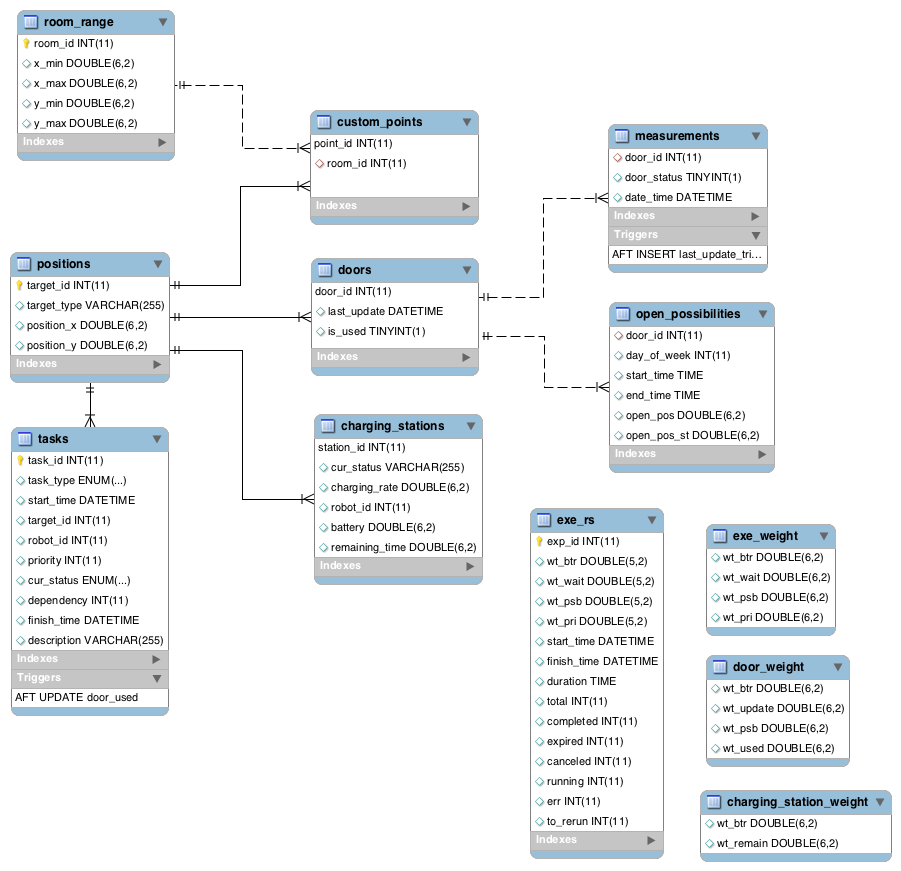
\includegraphics[width = 0.8\textwidth]{content/images/ch4/database_er.png}
 \caption{Database Entity Relationship Diagram}
 \label{fig:database_er}
 \end{figure} 

%\begin{table}
%\centering
%\begin{tabular}{|c|c|c|} 
%\hline
%Table Name & Example & Explaination \\ \hline
%measurements & Table \ref{tab:db_measurement_result} & measurement result with timestamp \\ \hline
%doors & Table \ref{tab:db_doors} & door information \\ \hline
%tasks & Table \ref{tab:db_task_table} & task specifications \\ \hline 
%exe\_rs & Table \ref{tab:exp_decision_variables} & ``navigation tasks'' experiment result \\ \hline
%env\_rs & Table \ref{tab:enviroment_experiment_result} & ``gather enviroment information task'' experiment result \\ \hline
%open\_possibilities & Table \ref{tab:db_open_possibilities} & open possibilities table for different time slots and weekdays \\ \hline
%... & ... & ... \\ \hline
%\end{tabular}
%\caption{Tables in Database}
%\label{tab:tables_in_database}
%\end{table}



\section{Procedure}
\label{sec:task_scheduling_procedure}
As stated in Chapter 3, the goal of task scheduling is finishing all tasks as soon as possible while keeping the cost as low as possible. 
The task assignment and execution has two levels. \cite{Ivan2017} the task, and the path planner solves a planning problem. It takes an occupancy grid, a specific robot, and a set of task specifications. It generates trajectories for each task under the assumption that there are no dynamic obstacles (including other robots). According to those trajectories and task specifications, the lowest cost task will be assigned to the robot.
At the dynamic level, after each robot receives a task, it runs a navigation stack to execute this task stepwise. Each robot computes a local trajectory but takes into account dynamic obstacles.
The process of the robot task scheduling system is as follows.

\subsection{Centralized Pool}

\paragraph{Handle task Request}
With robot statuses such as positions and available battery provided by robots, the multi-robot task scheduling module in the architecture should perform multi-robot task scheduling. 
When the centralized pool receives a task request (Table \ref{tab:request_message}) from a robot, the multi-robot task scheduling module in the architecture. The implementation of task scheduling is shown in Figure \ref{fig:centralized_task_scheduling}. 

\begin{figure}
 \centering
 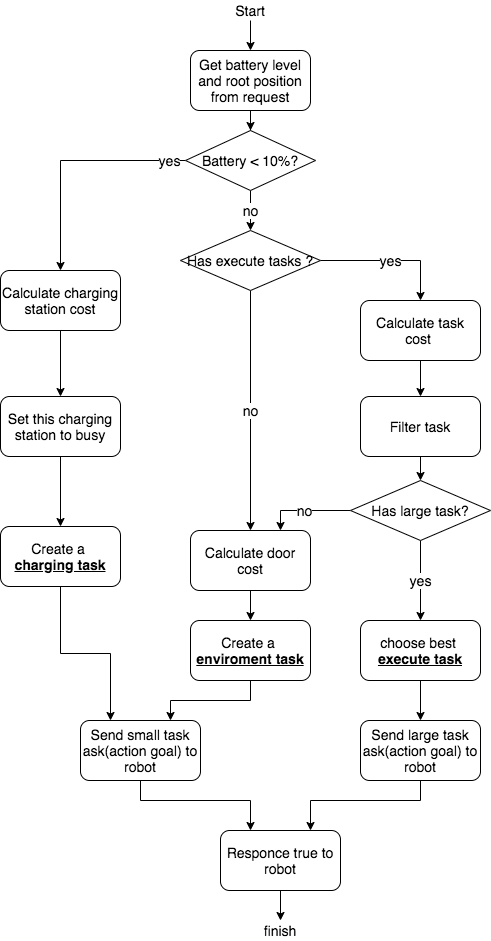
\includegraphics[width = 0.6\textwidth]{content/images/ch4/centralized_task_select.drawio.png}
 \caption{Centralized Pool Task Allocation}
 \label{fig:centralized_task_scheduling}
\end{figure}

\paragraph{Handle Task Feedback.}
When the centralized pool receives a task feedback (Table \ref{tab:feedback_message}) that contains a new measurement result from robot, it will add a record in ``measurement table'' and update ``open possibilities table'' in database (Table \ref{tab:db_open_possibilities}).

\paragraph{Handle Task Result.}
When the centralized pool receives a task result (Table \ref{tab:result_message}), it updates status column in ``tasks'' table in database. 
To make the robot complete the task as much as possible, whenever an ``navigation task'' failed, its start time will be delayed, and its priority will be increased by one until it exceeds the maximum and is marked as ``Failed''.
(Figure \ref{fig:centralized_task_handle}).


\begin{figure}
 \centering
 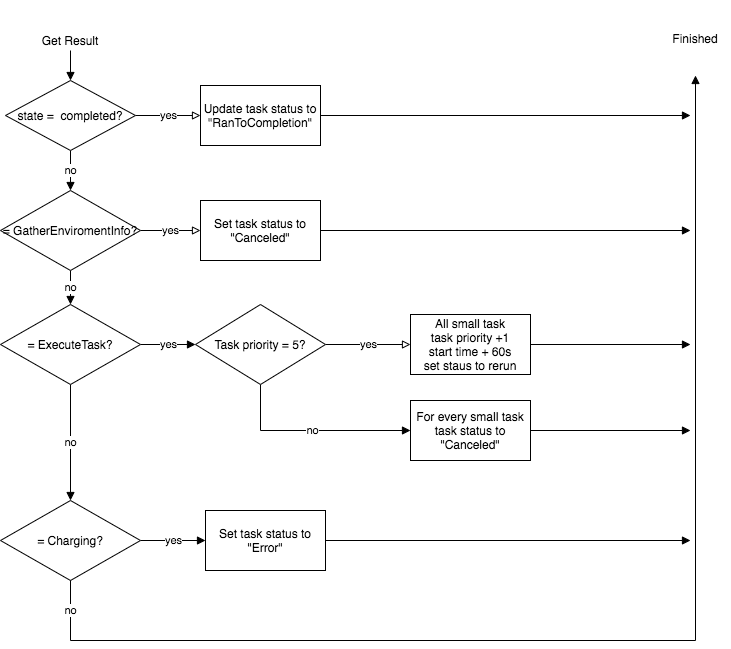
\includegraphics[width = 0.7\textwidth]{content/images/ch4/centralized_task_result.drawio.png}
 \caption{Centralized Pool Handle Task Result}
 \label{fig:centralized_task_handle}
 \paragraph{Task Status Explanation}
 \begin{itemize} 
 \item \textbf{Succeeded.} Robot successfully moved to the goal position and completed the task.
 \item \textbf{Error.} An error that cannot be corrected by itself occurred and the system requires manual restart. For example, a robot failed charging.
 \item \textbf{Failed.} A Task failed. Reasons of task failure includes: The robot was not able to move to goal positions or process robot action(\ref{fig:system_architecture}). 
 \item \textbf{To rerun.} If an ``navigation tasks'' failed, its priority was increased. The task is marked as ``to rerun task'' for a future scheduling by task scheduling module.
 \end{itemize} 
\end{figure}


\subsection{Robot}

\paragraph{Robot Process Tasks}
When the task queue(Figure \ref{fig:system_architecture}) in a robot is empty, the robot requests a new task. If the robot gets a ``charging task'', it will move to the position of charging station(Figure \ref{fig:door_station}) and interact with charging station node (Chapter \ref{sec:charging_station}).
When a robot gets an ``navigation tasks'' which is a complex task, it will move to all goals in order.
When a robot gets a ``gather information'' task, it will move to the door's position.
During task processing, the timer checks the status of the navigation stack periodically. If any errors occur, the robot sends a failed result with the description to the centralized pool. 
When all tasks are completed without error, the robot will send the ``Succeeded'' result to the centralized pool.


\begin{figure}
 \centering
 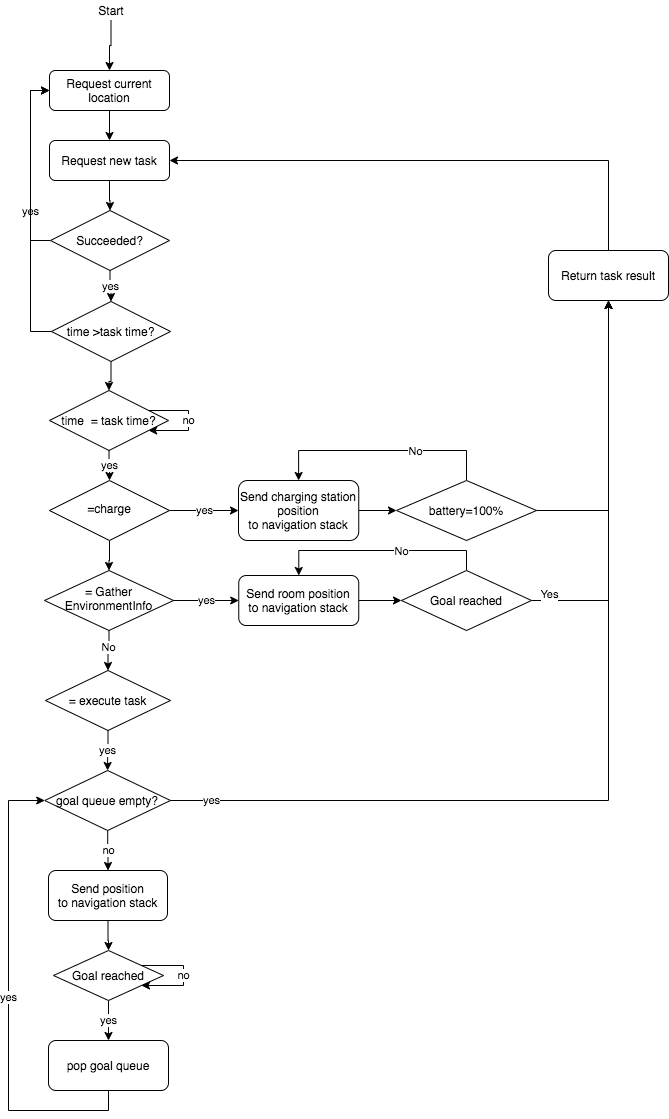
\includegraphics[width = 0.7\textwidth]{content/images/ch4/robot_process_task.drawio.png}
 \caption{Robot Process Task }
 \label{fig:task_process_robot}
\end{figure}


\begin{figure}
 \centering
 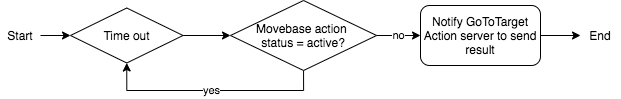
\includegraphics[width = 0.7\textwidth]{content/images/ch4/robot_timer.drawio.png}
 \caption{Robot Timer}
 \label{fig:robot_timer}
\end{figure}

\begin{figure}
 \centering
 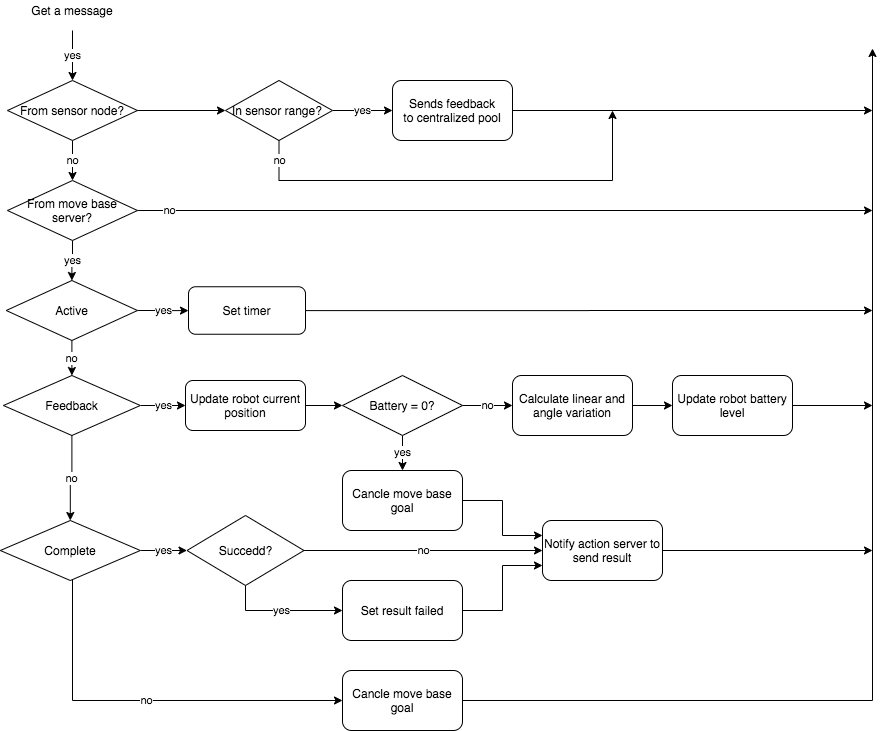
\includegraphics[width = 0.7\textwidth]{content/images/ch4/robot_message.drawio.png}
 \caption{Robot Handle Message}
 \label{fig:robot_handle_message}
\end{figure}

\paragraph{Robot Handle Messages}
While a robot is processing a task, it listens to door sensors and forwards measurement data to the centralized pool. 
Besides messages from sensors, it also receives messages from the ``move\_base'' node. The details of robot message handling are shown in Figure \ref{fig:robot_handle_message}.

\subsection{Charging Station}
\label{sec:charging_station}
The charging station consists of a charging station node and ``charging station'' table in database (Table \ref{fig:database_er}). 

A charging station has four states: ``Free'', ``Charging'' and ``Charging finished''. Its initial state is ``Free''. When a robot arrives at the charging station, it will start interacting with the charging station node (Figure \ref{fig:charging_station_message}). 
Once the charging station receives robot information, its state will be changed to ``Charging'' and its ``battery level'' will be increased, and its ``remaining time'' will be decreased (Figure \ref{fig:charging_station_event}). 
Once finishing charging, its status will be set to ``Charging finished''. When the robot leaves the charging station, its status will be set to ``Free''. 

\begin{figure}
 \centering
 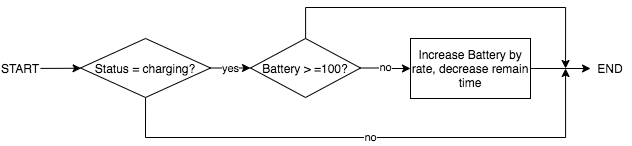
\includegraphics[width = 0.7\textwidth]{content/images/ch4/charging_station_charging_event.drawio.png}
 \caption{Charging Station Scheduled Charging Event in Database}
 \label{fig:charging_station_event}
\end{figure}

\begin{figure}
 \centering
 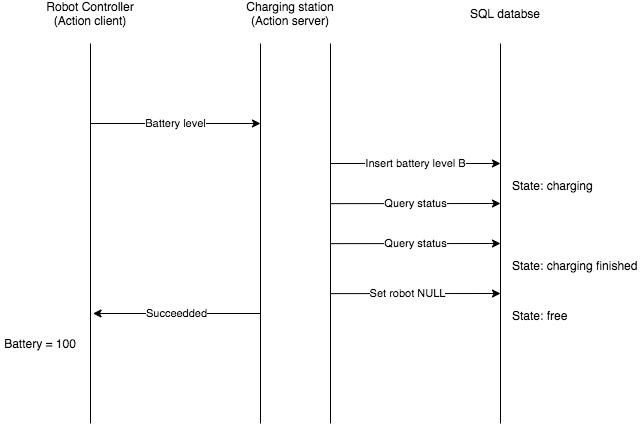
\includegraphics[width = 0.9\textwidth]{content/images/ch4/charging_station_message.drawio.png}
 \caption{Charging Station Message}
 \label{fig:charging_station_message}
\end{figure}

